\documentclass{exam}
\usepackage{mainExam}

\title{Interrogation de Cours}
\date{27 Septembre 2024}
\author{Seconde 9}

\begin{document}

\maketitle
\instructions
\begin{questions}
\question Effectuer les calculs fractionnaires suivants.
\begin{parts}
\part $A = \dfrac{6}{8} + \dfrac{6}{8} \times \dfrac{5}{3}$
\part $B = \dfrac{3}{2} \times \dfrac{3}{5} + \dfrac{7}{2}$
\part $C = \dfrac{7}{3} \times \dfrac{3}{8} - \dfrac{5}{3}$
\makeemptybox{6cm}
\end{parts}

\question
\begin{parts}
\part Nommer les trois caractéristiques d'un vecteur:
\makeemptybox{2cm}

\part Dans cette figure, les trois triangles $ABD$, $BCE$ et $DEF$ sont équilatéraux.
\begin{center}
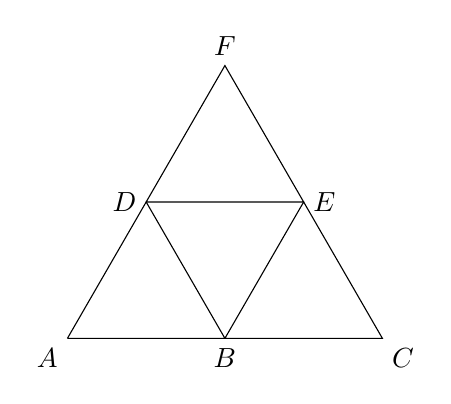
\begin{tikzpicture}
\draw (0,0) node[below left] {$A$} -- ++(0:2) node[below] {$B$} -- ++(120:2) node[left] {$D$} -- ++(240:2);
\draw (2,0) -- ++(0:2) node[below right] {$C$} -- ++(120:2) node[right] {$E$} -- ++(240:2);
\draw (0,0)  ++(60:2) -- ++(0:2) -- ++(120:2) node[above] {$F$} -- ++(240:2);
\end{tikzpicture}
\end{center}
Pour chaque vecteur proposé, nommer deux vecteurs égaux à celui-ci:
\begin{subparts}
\subpart $\vect{AB}$
\subpart $-\vect{BC}$
\end{subparts}
\makeemptybox{3cm}
\end{parts}

\end{questions}

\newpage

\maketitle

\instructions

\begin{questions}
\question Effectuer les calculs de fractions suivants.
\begin{parts}
\part $D = \dfrac{7}{8} + \dfrac{3}{8} \times \dfrac{4}{2}$ 
\part $E = \dfrac{7}{4} - \dfrac{5}{4} \times \dfrac{2}{9}$
\part $F = \dfrac{9}{5} \times \dfrac{2}{8} - \dfrac{2}{5}$
\end{parts}
\makeemptybox{6cm}
\question
\begin{parts}
\part Nommer les trois caractéristiques d'un vecteur:
\makeemptybox{2cm}

\part Dans cette figure, les trois triangles $ABD$, $BCE$ et $DEF$ sont équilatéraux.
\begin{center}
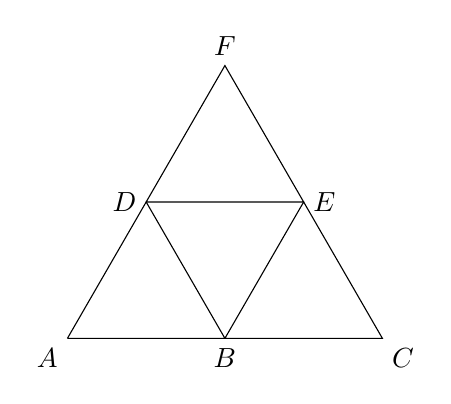
\begin{tikzpicture}
\draw (0,0) node[below left] {$A$} -- ++(0:2) node[below] {$B$} -- ++(120:2) node[left] {$D$} -- ++(240:2);
\draw (2,0) -- ++(0:2) node[below right] {$C$} -- ++(120:2) node[right] {$E$} -- ++(240:2);
\draw (0,0)  ++(60:2) -- ++(0:2) -- ++(120:2) node[above] {$F$} -- ++(240:2);
\end{tikzpicture}
\end{center}
Pour chaque vecteur proposé, nommer deux vecteurs égaux à celui-ci:
\begin{subparts}
\subpart $\vect{EF}$
\subpart $-\vect{DF}$
\end{subparts}
\makeemptybox{3cm}
\end{parts}
\end{questions}

\end{document}